%------------------------------------------------
%-----session 5: Applications, Chih Yun Pai------
%------------------------------------------------

\section{Applications}
\begin{frame}
\huge\frametitle{Section 5: Applications}
\centering
Section 5: Applications
\par
\end{frame}
%------------------------------------------------
%Quick Review
%------------------------------------------------
\begin{frame}
\frametitle{Quick Review}

What we get so far... \newline\newline

Logistic Regression hypothesis: $h_\theta(x)=\frac{1}{1+e^{-\theta^Tx}}$\newline\newline

Optimization: Gradient Descent / Newton Method\newline\newline

Regularization\newline\newline

\end{frame}

%------------------------------------------------
%Logistic Regression as binary classifier-1
%------------------------------------------------
\subsection{LR for Linearly Separable Dataset}
\begin{frame}
\frametitle{Logistic Regression as Binary Classifier}
Problem: Predict whether a student gets admitted into a university, given two historical exams data.\newline\newline
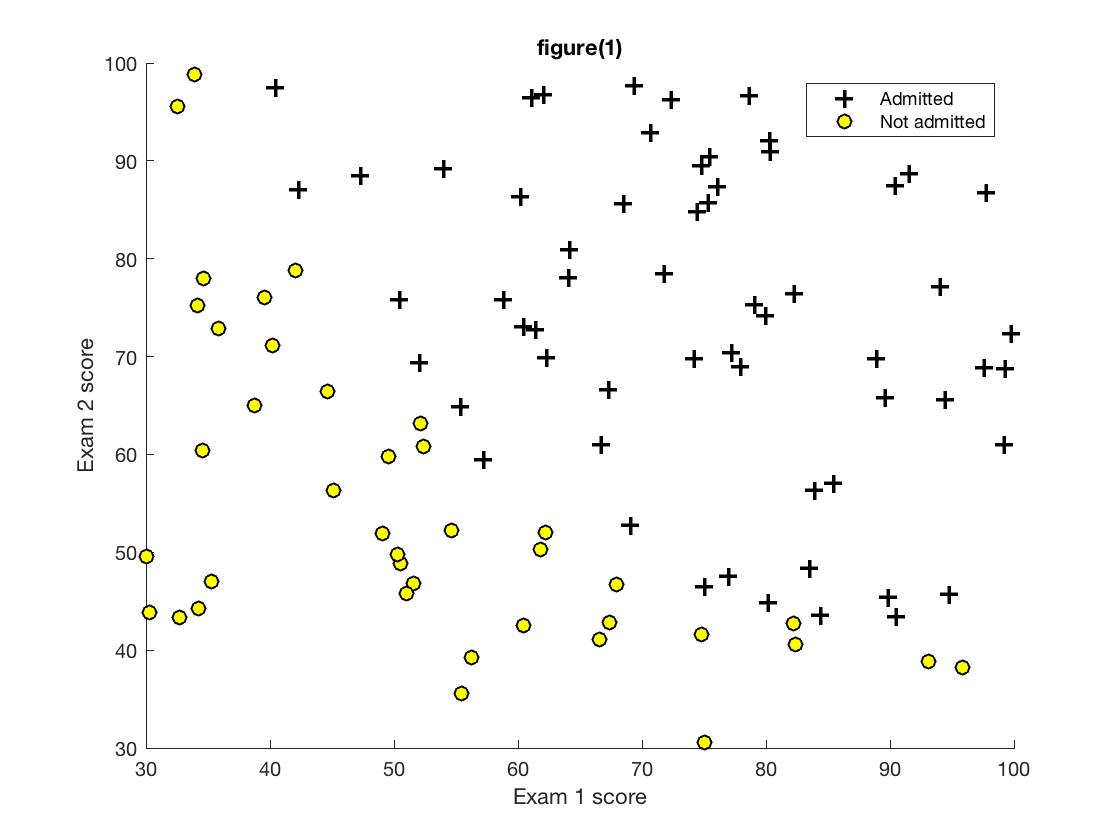
\includegraphics[width=4cm,height=5cm,keepaspectratio]{pictures/1_plotData1}\newline
Labels: y=1: Admitted / y=0: Not admitted\newline\newline
Logistic model: $h_\theta(x)=\frac{1}{1+e^{-\theta^Tx}}$\newline\newline
\end{frame}

%------------------------------------------------
%Logistic Regression as binary classifier-2
%------------------------------------------------
\subsection{LR for Nonlinearly Separable Dataset}
\begin{frame}
\frametitle{Logistic Regression as Binary Classifier}
Cost function without regularization: \newline\newline
$J(\theta)=\frac{1}{n}\sum\limits_{i=1}^n[-y^{(i)}*log(h_\theta(x^{(i)}))-(1-y^{(i)})*log(1-h_\theta(x^{(i)})]$\newline\newline
Optimized by Gradient Descent\newline\newline
Training Accuracy: 89\%
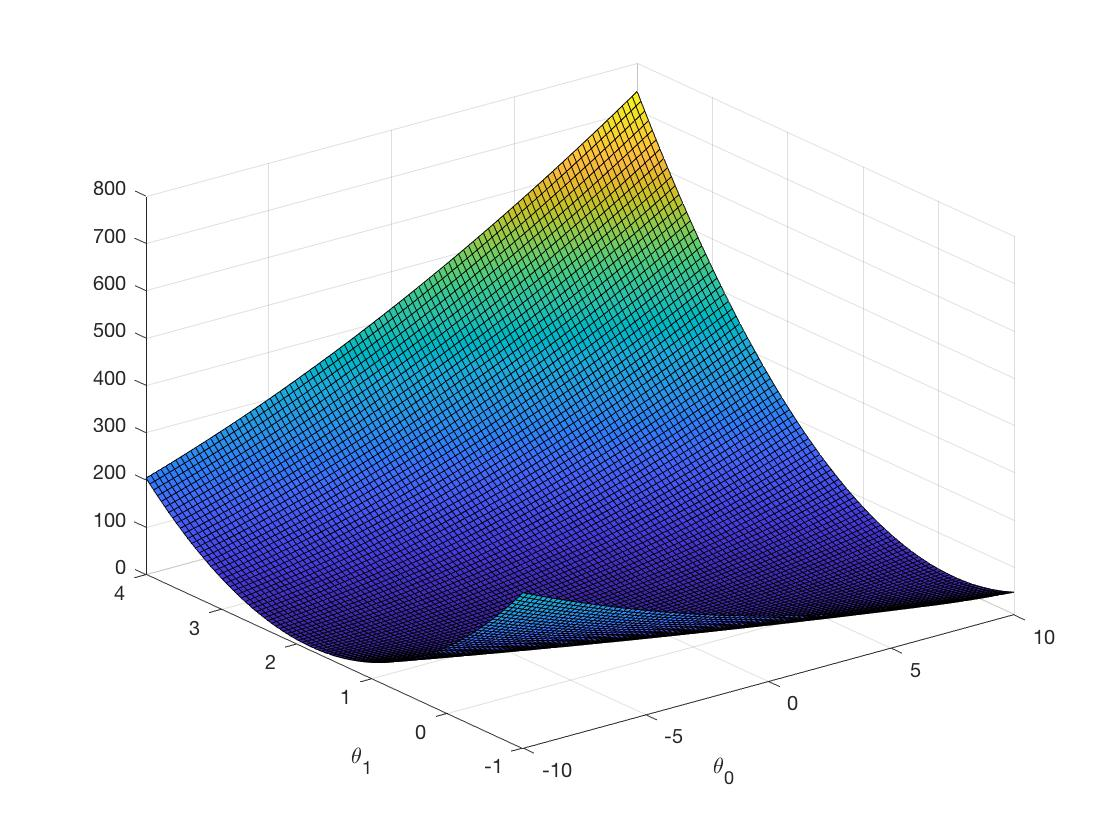
\includegraphics[width=5cm,height=5cm,keepaspectratio]{pictures/0_optimization_result_in_3-d_graph}
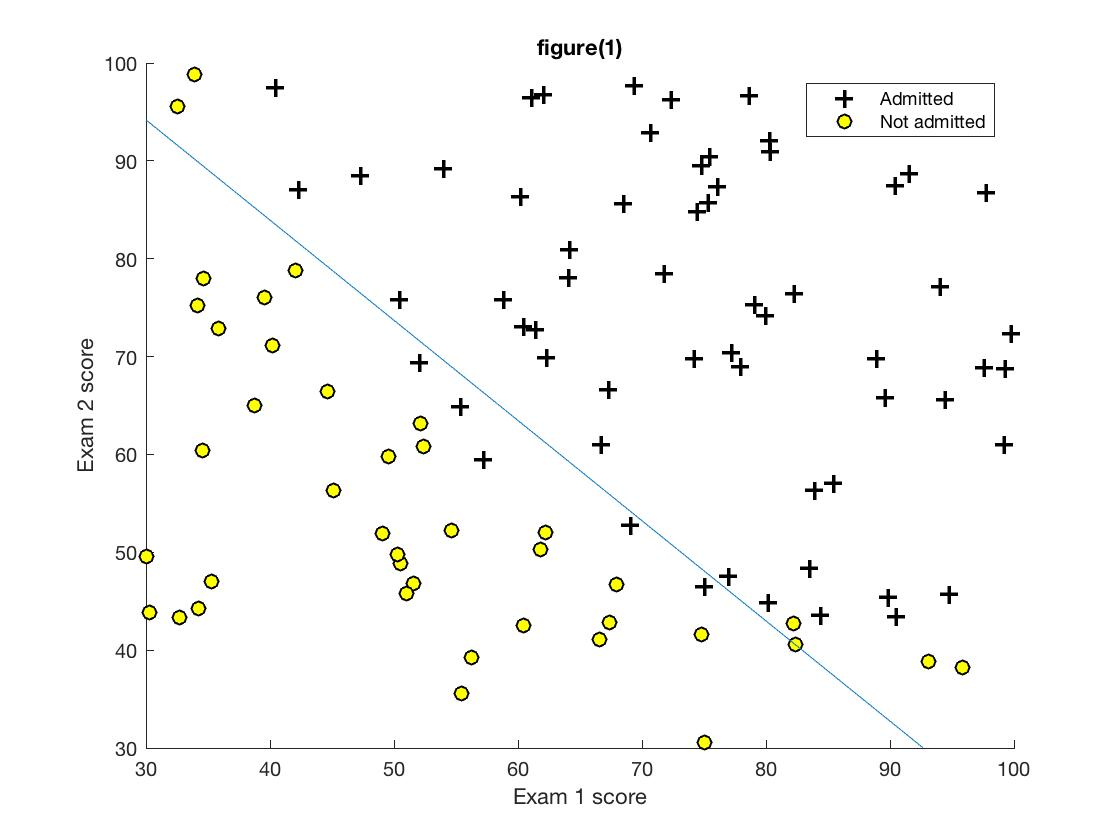
\includegraphics[width=5cm,height=5cm,keepaspectratio]{pictures/2_plotData1_decision_boundary}
\end{frame}

%------------------------------------------------
%Logistic Regression as binary classifier with Regularization-1
%------------------------------------------------
\begin{frame}
\frametitle{Logistic Regression as Binary Classifier with Regularization}
Problem: Predict whether a product of Microchip Manufacturing is malfunction, given 2 kind of tests score. Labels: y=1 pass / y=0 fail.\newline\newline
Logistic model: $h_\theta(x)=\frac{1}{1+e^{-\theta^Tx}}$\newline\newline
Cost function with regularization: \newline\newline
$J(\theta)=\frac{1}{n}\sum\limits_{i=1}^n[-y^{(i)}*log(h_\theta(x^{(i)}))-(1-y^{(i)})*log(1-h_\theta(x^{(i)})]+\frac{\lambda}{2n}\sum\limits_{j=1}^d\theta_j^2$\newline\newline
Feature Transformation: $Z(x)=[1,x_1,x_2,x_1^2,x_2^2,x_1x_2,...,x_1x_2^5,x_2^6]^T$\newline\newline
Optimized by Gradient Descent\newline\newline

\end{frame}

%------------------------------------------------
%Logistic Regression as binary classifier with Regularization-2
%------------------------------------------------
\begin{frame}
\frametitle{Logistic Regression as Binary Classifier with Regularization}

Training Accuracy: \newline\newline

\begin{figure}[h!]

\begin{subfigure}{.3\textwidth}
  \centering
  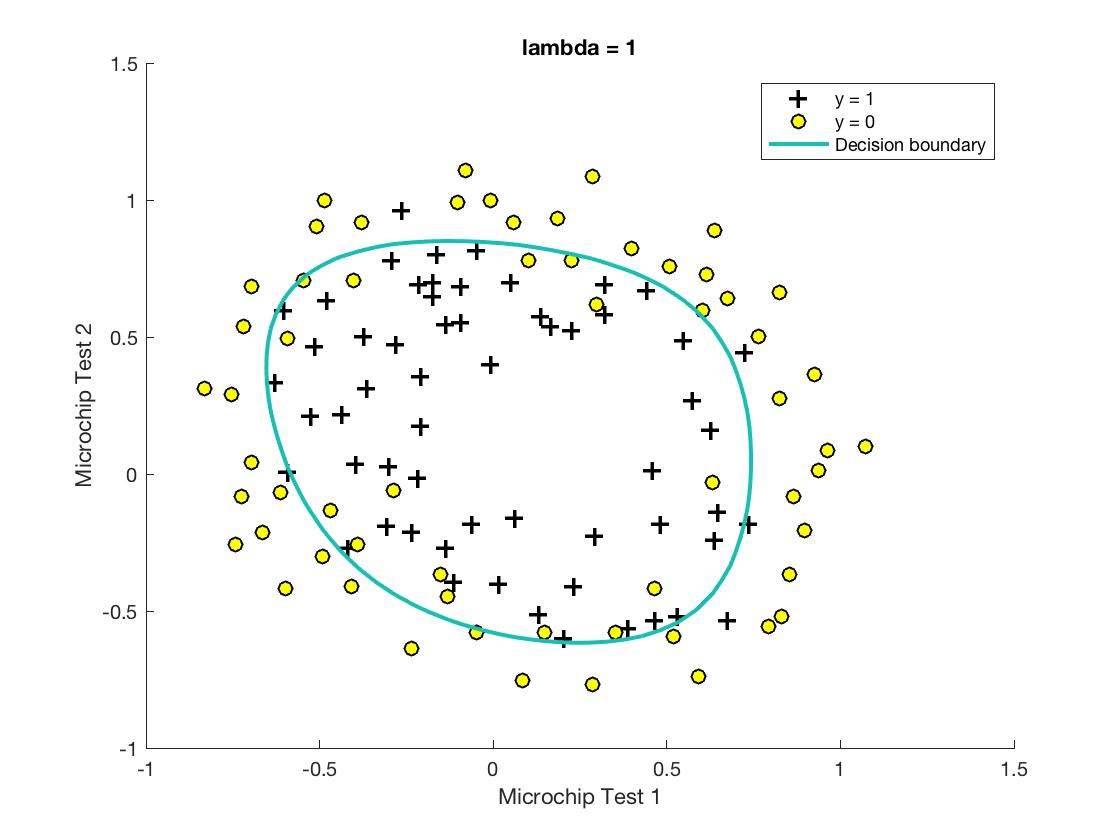
\includegraphics[scale = 0.1]{pictures/4_plotData2_lambda_1}
  \caption{$\lambda=1$:\\ accuracy = 83\% \\ Good fitting}
  \label{fig:sub1}
\end{subfigure}
\begin{subfigure}{.3\textwidth}
  \centering
  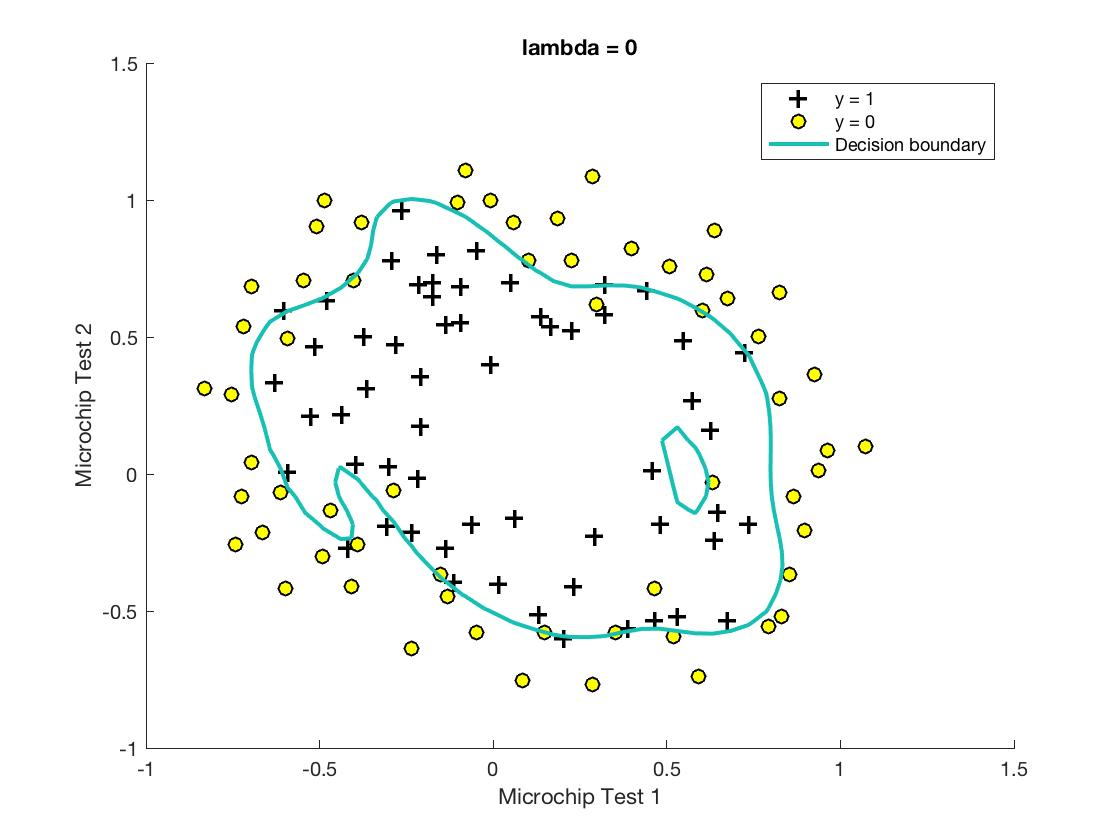
\includegraphics[scale = 0.1]{pictures/5_plotData2_lambda_0_overfitting}
  \caption{$\lambda=0$:\\ accuracy = 87\% \\ Over-fitting}
  \label{fig:sub2}
\end{subfigure}
\begin{subfigure}{.3\textwidth}
  \centering
  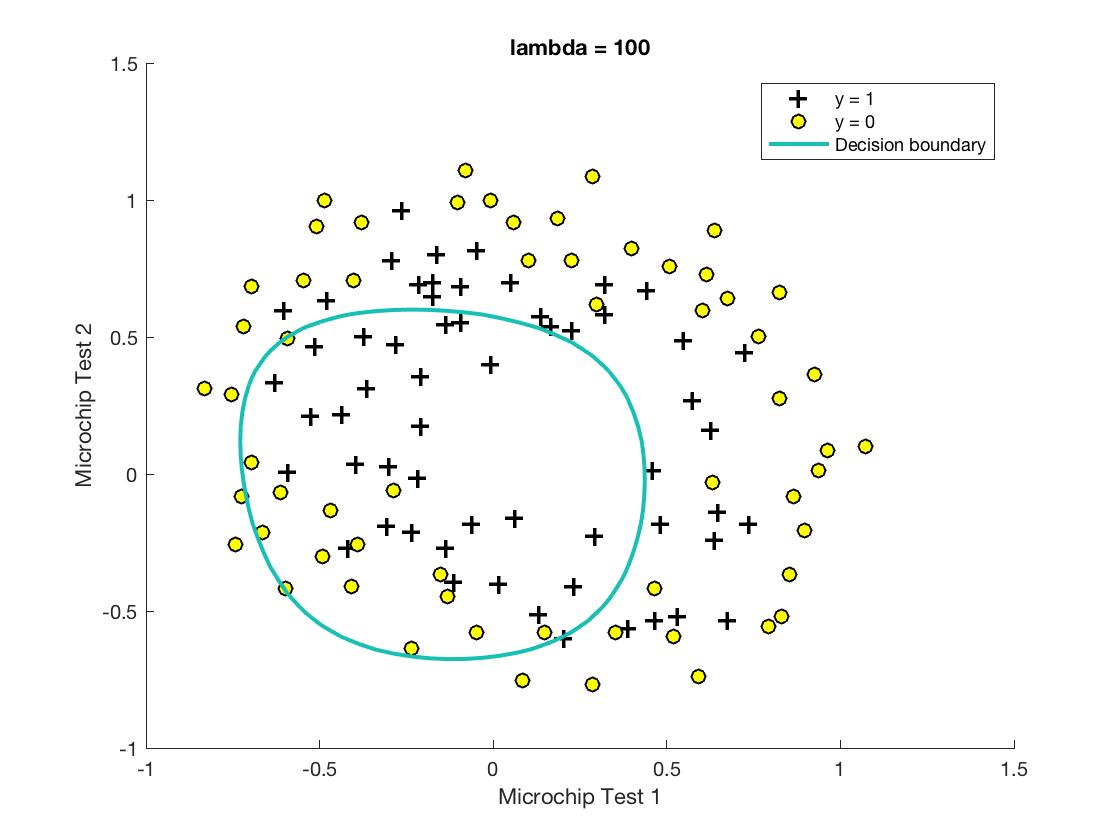
\includegraphics[scale = 0.1]{pictures/6_plotData2_lambda_100_underfitting}
  \caption{$\lambda=100$:\\ accuracy = 61\% \\ Under-fitting}
  \label{fig:sub2}
\end{subfigure}
\end{figure}

\end{frame}

%------------------------------------------------
%Handwritten Digit Recognition
%------------------------------------------------
\subsection{Applications: Handwritten Digit Recognition}
\begin{frame}
\frametitle{Handwritten Digit Recognition}
Problem: Recognize handwritten digits (from 0-9)\newline\newline
Dataset: 5000 20 pixel by 20 pixel greyscale images, 5000 labels \newline\newline
X: 5,000 $\times$400 matrix\newline\newline
Y: 5,000 $\times$1 vector $\in {0,1,...,9}$
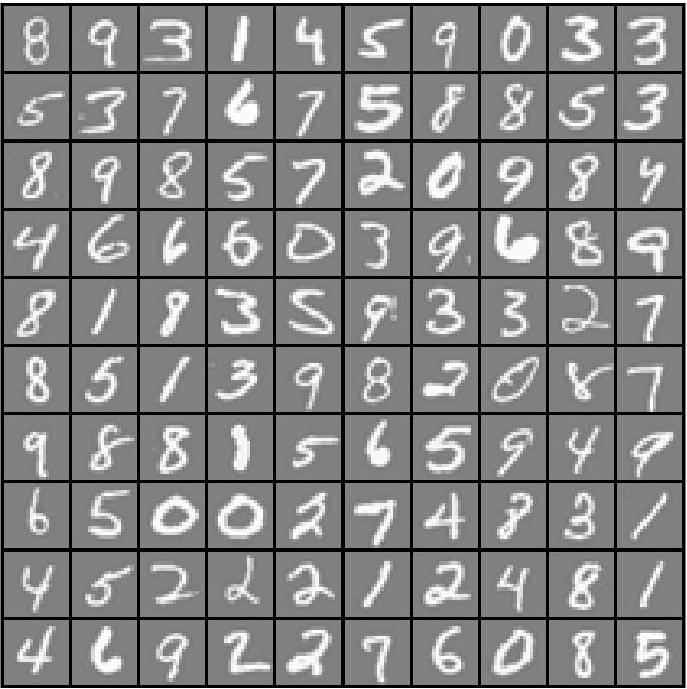
\includegraphics[width=4cm,keepaspectratio]{pictures/7_digits}
\end{frame}

%------------------------------------------------
%Handwritten Digit Recognition - Model
%------------------------------------------------

\begin{frame}
\frametitle{Handwritten Digit Recognition - Model}
Model:\newline
- Logistic Regression hypothesis: $h_\theta(x)=\frac{1}{1+e^{-
\theta^Tx}}$\newline
- One vs All multi-class classification: $h_\theta^{(c)}=P(y=c|x;\theta), c=1,...,10$\newline
- Prediction: $\underset{c}max$ $h_\theta^{(c)}(x)$\newline
- Neural Network  (one hidden layer, 25 units), Optimization: Back-propagation with Gradient Descent\newline
\begin{centering}
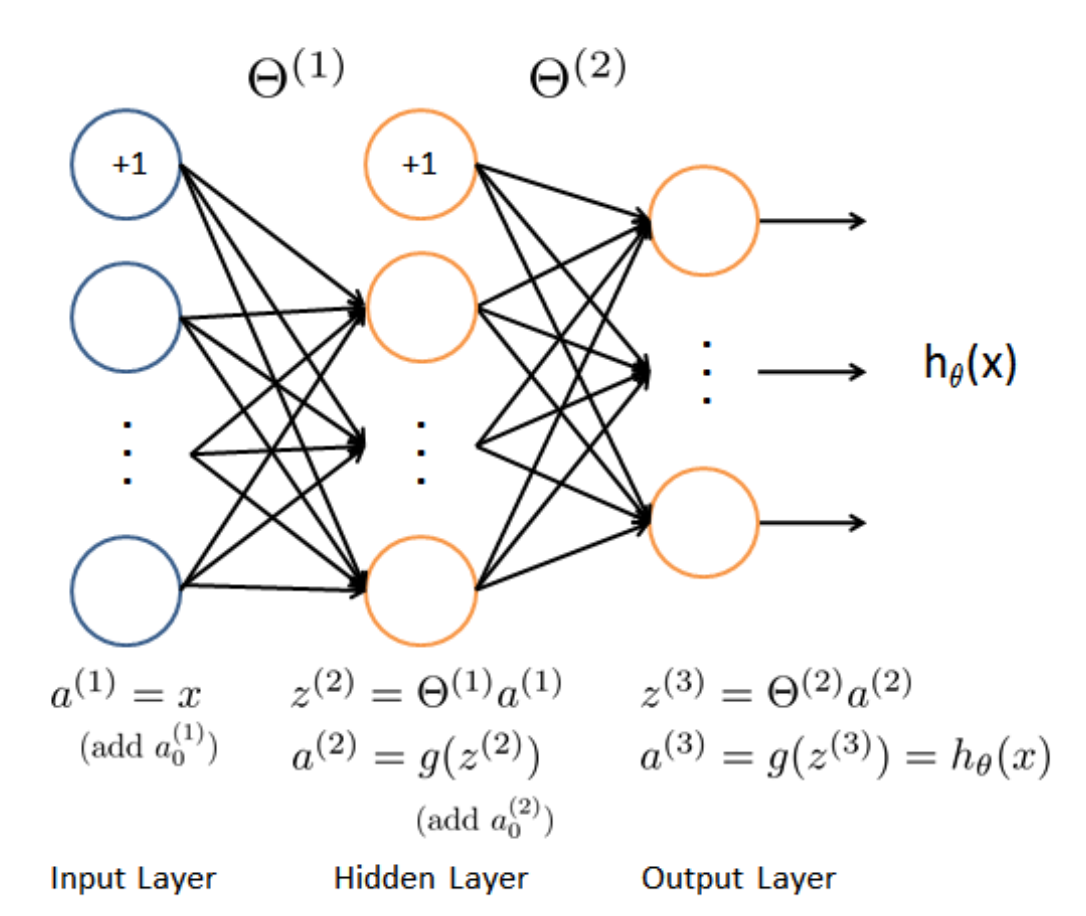
\includegraphics[width=5cm,keepaspectratio]{pictures/8_Neural_network_model}
\end{centering}
\end{frame}

%------------------------------------------------
%Handwritten Digit Recognition - Result
%------------------------------------------------
\begin{frame}
\frametitle{Handwritten Digit Recognition - Result}
\begin{itemize}
\item Hidden layer units visualization \newline\newline
\begin{figure}
\begin{centering}
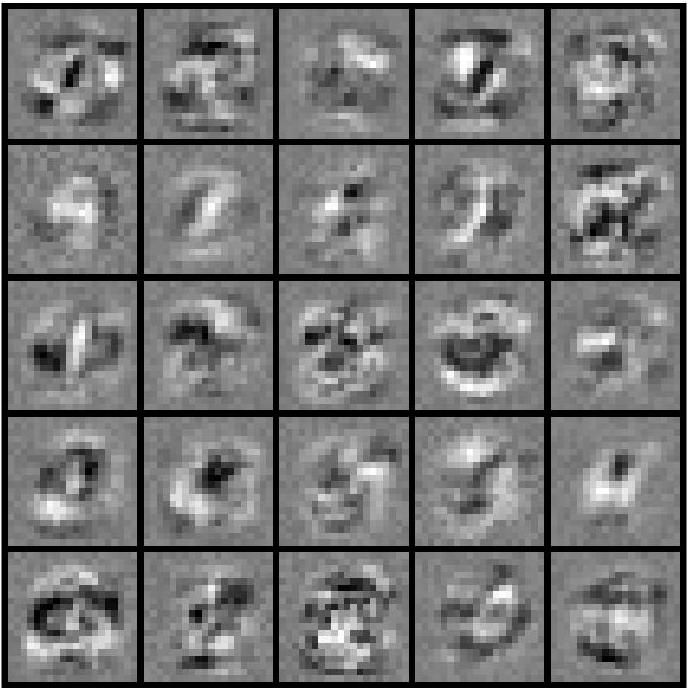
\includegraphics[width=4cm,keepaspectratio]{pictures/9_Visualizeing_hidden_layer}
\end{centering}
\end{figure}
\item Training Accuracy:\newline
97.52\% without regularization, $\lambda=0$\newline
95.36\% with regularization, $\lambda=1$ \newline
\end{itemize}
\end{frame}
%------------------------------------------------

